\documentclass[12pt]{article}

% style
\setlength{\parindent}{0pt}
\usepackage[left=2.5cm,top=2cm,right=2.5cm,bottom=2cm,a4paper]{geometry}
\usepackage{fancyhdr}
\pagestyle{fancy}
\lhead{Team 4: TeamR2D2}
\rhead{Overzicht ontwerpspecificaties}
\renewcommand{\headrulewidth}{0.4pt}
\usepackage{lscape}
\usepackage{hyperref}
\usepackage{graphicx}
\usepackage{amsmath, amssymb, amsthm}

\usepackage{siunitx}
\usepackage[dutch]{babel}

\usepackage{translator}

\usepackage{longtable}
\usepackage{booktabs}
\usepackage{enumitem}
\usepackage{array}

\setlist[itemize]{noitemsep, topsep=0pt, leftmargin=*}


\begin{document}



\uselanguage{Dutch}
\languagepath{Dutch}
\providetranslation[to=Dutch]{Figure}{Figuur}



\section*{Overzicht ontwerpspecificaties}
De verkeerslichten kunnen interpreteren: stoppen bij een rood licht, doorrijden bij een groen licht

\begin{itemize}
\item Hoogte middelpunt verkeerslicht: $75mm$
\item Knipperfrequentie verkeerslicht: $1Hz$
\item Technische tekening van een verkeerslicht te zien op  \ref{fig: verkeerslicht}
\end{itemize}
\bigskip



Een geïmplementeerd traject kunnen volgen / stoplijn detecteren

\begin{itemize}
\item Ondergrond: donker / helder
\item Kleur van de lijnen: helder / donker 
\item Breedte volglijn: $25mm$
\item Breedte stoplijn: $50mm$
\item Afstand tussen kruispunten: $1000mm$
\item Figuur \ref{fig: kruispunt} toont het bovenaanzicht van een kruispunt
\end{itemize}
\bigskip


Commando's van een computer kunnen volgen

\begin{itemize}
\item Noodstop op afstand uitvoeren
\end{itemize}

\bigskip

De auto moet aan een bepaald budget voldoen
\begin{itemize}
\item Virtueel budget: $3500$
\item Te besteden aan het aankopen van materiaal beschikbaar op:  	http://www.irkulak.be/po2/

\item Te besteden aan het 3D-printen van eigen ontwerpen
\end{itemize}
\bigskip
Het volledige traject foutloos kunnen afleggen met een aanvaardbaar tempo
\begin{itemize}
	\item Maximumbreedte wagen: $250mm$
	\item Maximumhoogte wagen: $300mm$
	\item Minimumhoogte wagen: $75mm$
	
	
\end{itemize}
\bigskip
\begin{figure}
	\centering
	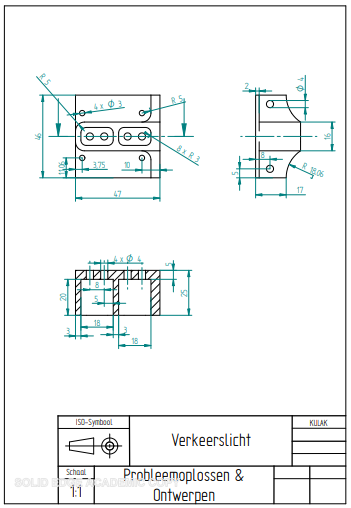
\includegraphics[width=.8\textwidth]{verkeerslicht}
	\caption{Technische tekening verkeerslicht, opgehaald van \cite{artikel1} }
	\label{fig: verkeerslicht}
\end{figure}
\bigskip
\begin{figure}
	\centering
	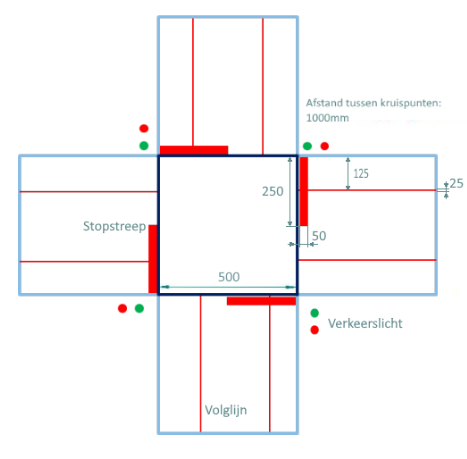
\includegraphics[width=.8\textwidth]{bovenaanzichtkruispunt}
	\caption{Bovenaanzicht kruispunt met relevante maten en items, aangepast vanuit \cite{Smart}.
	}
	\label{fig: kruispunt}
\end{figure}






\bibliography{ontwerps}
\bibliographystyle{unsrt}


\end{document}